\documentclass[twoside]{book}

% Packages required by doxygen
\usepackage{fixltx2e}
\usepackage{calc}
\usepackage{doxygen}
\usepackage[export]{adjustbox} % also loads graphicx
\usepackage{graphicx}
\usepackage[utf8]{inputenc}
\usepackage{makeidx}
\usepackage{multicol}
\usepackage{multirow}
\PassOptionsToPackage{warn}{textcomp}
\usepackage{textcomp}
\usepackage[nointegrals]{wasysym}
\usepackage[table]{xcolor}

% Font selection
\usepackage[T1]{fontenc}
\usepackage[scaled=.90]{helvet}
\usepackage{courier}
\usepackage{amssymb}
\usepackage{sectsty}
\renewcommand{\familydefault}{\sfdefault}
\allsectionsfont{%
  \fontseries{bc}\selectfont%
  \color{darkgray}%
}
\renewcommand{\DoxyLabelFont}{%
  \fontseries{bc}\selectfont%
  \color{darkgray}%
}
\newcommand{\+}{\discretionary{\mbox{\scriptsize$\hookleftarrow$}}{}{}}

% Page & text layout
\usepackage{geometry}
\geometry{%
  a4paper,%
  top=2.5cm,%
  bottom=2.5cm,%
  left=2.5cm,%
  right=2.5cm%
}
\tolerance=750
\hfuzz=15pt
\hbadness=750
\setlength{\emergencystretch}{15pt}
\setlength{\parindent}{0cm}
\setlength{\parskip}{3ex plus 2ex minus 2ex}
\makeatletter
\renewcommand{\paragraph}{%
  \@startsection{paragraph}{4}{0ex}{-1.0ex}{1.0ex}{%
    \normalfont\normalsize\bfseries\SS@parafont%
  }%
}
\renewcommand{\subparagraph}{%
  \@startsection{subparagraph}{5}{0ex}{-1.0ex}{1.0ex}{%
    \normalfont\normalsize\bfseries\SS@subparafont%
  }%
}
\makeatother

% Headers & footers
\usepackage{fancyhdr}
\pagestyle{fancyplain}
\fancyhead[LE]{\fancyplain{}{\bfseries\thepage}}
\fancyhead[CE]{\fancyplain{}{}}
\fancyhead[RE]{\fancyplain{}{\bfseries\leftmark}}
\fancyhead[LO]{\fancyplain{}{\bfseries\rightmark}}
\fancyhead[CO]{\fancyplain{}{}}
\fancyhead[RO]{\fancyplain{}{\bfseries\thepage}}
\fancyfoot[LE]{\fancyplain{}{}}
\fancyfoot[CE]{\fancyplain{}{}}
\fancyfoot[RE]{\fancyplain{}{\bfseries\scriptsize Generated by Doxygen }}
\fancyfoot[LO]{\fancyplain{}{\bfseries\scriptsize Generated by Doxygen }}
\fancyfoot[CO]{\fancyplain{}{}}
\fancyfoot[RO]{\fancyplain{}{}}
\renewcommand{\footrulewidth}{0.4pt}
\renewcommand{\chaptermark}[1]{%
  \markboth{#1}{}%
}
\renewcommand{\sectionmark}[1]{%
  \markright{\thesection\ #1}%
}

% Indices & bibliography
\usepackage{natbib}
\usepackage[titles]{tocloft}
\setcounter{tocdepth}{3}
\setcounter{secnumdepth}{5}
\makeindex

% Hyperlinks (required, but should be loaded last)
\usepackage{ifpdf}
\ifpdf
  \usepackage[pdftex,pagebackref=true]{hyperref}
\else
  \usepackage[ps2pdf,pagebackref=true]{hyperref}
\fi
\hypersetup{%
  colorlinks=true,%
  linkcolor=blue,%
  citecolor=blue,%
  unicode%
}

% Custom commands
\newcommand{\clearemptydoublepage}{%
  \newpage{\pagestyle{empty}\cleardoublepage}%
}

\usepackage{caption}
\captionsetup{labelsep=space,justification=centering,font={bf},singlelinecheck=off,skip=4pt,position=top}

%===== C O N T E N T S =====

\begin{document}

% Titlepage & ToC
\hypersetup{pageanchor=false,
             bookmarksnumbered=true,
             pdfencoding=unicode
            }
\pagenumbering{alph}
\begin{titlepage}
\vspace*{7cm}
\begin{center}%
{\Large Space \\[1ex]\large 1 }\\
\vspace*{1cm}
{\large Generated by Doxygen 1.8.13}\\
\end{center}
\end{titlepage}
\clearemptydoublepage
\pagenumbering{roman}
\tableofcontents
\clearemptydoublepage
\pagenumbering{arabic}
\hypersetup{pageanchor=true}

%--- Begin generated contents ---
\chapter{R\+E\+A\+D\+ME}
\label{md__r_e_a_d_m_e}
\Hypertarget{md__r_e_a_d_m_e}
\input{md__r_e_a_d_m_e}
\chapter{Hierarchical Index}
\section{Class Hierarchy}
This inheritance list is sorted roughly, but not completely, alphabetically\+:\begin{DoxyCompactList}
\item \contentsline{section}{Game\+Object}{\pageref{class_game_object}}{}
\begin{DoxyCompactList}
\item \contentsline{section}{Bullet}{\pageref{class_bullet}}{}
\item \contentsline{section}{Earth}{\pageref{class_earth}}{}
\item \contentsline{section}{Satellite}{\pageref{class_satellite}}{}
\item \contentsline{section}{Trash}{\pageref{class_trash}}{}
\end{DoxyCompactList}
\end{DoxyCompactList}

\chapter{Class Index}
\section{Class List}
Here are the classes, structs, unions and interfaces with brief descriptions\+:\begin{DoxyCompactList}
\item\contentsline{section}{\hyperlink{class_bullet}{Bullet} }{\pageref{class_bullet}}{}
\item\contentsline{section}{\hyperlink{class_earth}{Earth} }{\pageref{class_earth}}{}
\item\contentsline{section}{\hyperlink{class_game_object}{Game\+Object} }{\pageref{class_game_object}}{}
\item\contentsline{section}{\hyperlink{class_satellite}{Satellite} }{\pageref{class_satellite}}{}
\item\contentsline{section}{\hyperlink{class_trash}{Trash} }{\pageref{class_trash}}{}
\end{DoxyCompactList}

\chapter{Class Documentation}
\hypertarget{class_bullet}{}\section{Bullet Class Reference}
\label{class_bullet}\index{Bullet@{Bullet}}


Inheritance diagram for Bullet\+:
\nopagebreak
\begin{figure}[H]
\begin{center}
\leavevmode
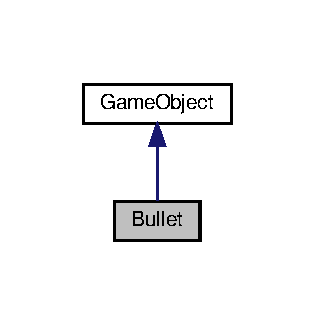
\includegraphics[width=151pt]{class_bullet__inherit__graph}
\end{center}
\end{figure}


Collaboration diagram for Bullet\+:
\nopagebreak
\begin{figure}[H]
\begin{center}
\leavevmode
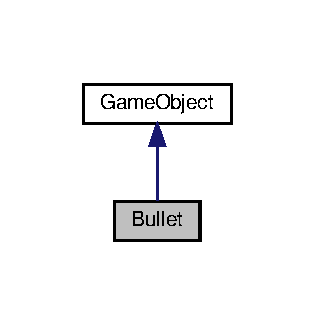
\includegraphics[width=151pt]{class_bullet__coll__graph}
\end{center}
\end{figure}
\subsection*{Public Member Functions}
\begin{DoxyCompactItemize}
\item 
\mbox{\Hypertarget{class_bullet_aaaf2d5b5a33b32f68a767c3905714dea}\label{class_bullet_aaaf2d5b5a33b32f68a767c3905714dea}} 
sf\+::\+Sprite \& {\bfseries get\+Sprite} ()
\item 
\mbox{\Hypertarget{class_bullet_a085bb7c0585ded8b8fb6fab17ea6d936}\label{class_bullet_a085bb7c0585ded8b8fb6fab17ea6d936}} 
float {\bfseries get\+VX} ()
\item 
\mbox{\Hypertarget{class_bullet_ac0c532a9810fea73f8cb68a4e9180b26}\label{class_bullet_ac0c532a9810fea73f8cb68a4e9180b26}} 
float {\bfseries get\+VY} ()
\item 
\mbox{\Hypertarget{class_bullet_a01f8720e8456eb80d49b82454e119620}\label{class_bullet_a01f8720e8456eb80d49b82454e119620}} 
void {\bfseries set\+VX} (float velocity\+\_\+x)
\item 
\mbox{\Hypertarget{class_bullet_ad16379f51f3ac3b55c3f8aa0710db3cb}\label{class_bullet_ad16379f51f3ac3b55c3f8aa0710db3cb}} 
void {\bfseries set\+VY} (float velocity\+\_\+y)
\item 
\mbox{\Hypertarget{class_bullet_ab96a969270f7c38d9e13d4e97800ef85}\label{class_bullet_ab96a969270f7c38d9e13d4e97800ef85}} 
{\bfseries Bullet} (int x, int y, float scale)
\end{DoxyCompactItemize}
\subsection*{Additional Inherited Members}


The documentation for this class was generated from the following files\+:\begin{DoxyCompactItemize}
\item 
bullet.\+h\item 
bullet\+\_\+obj.\+cpp\end{DoxyCompactItemize}

\hypertarget{class_earth}{}\section{Earth Class Reference}
\label{class_earth}\index{Earth@{Earth}}


Inheritance diagram for Earth\+:
\nopagebreak
\begin{figure}[H]
\begin{center}
\leavevmode
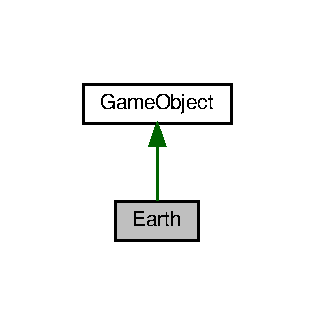
\includegraphics[width=151pt]{class_earth__inherit__graph}
\end{center}
\end{figure}


Collaboration diagram for Earth\+:
\nopagebreak
\begin{figure}[H]
\begin{center}
\leavevmode
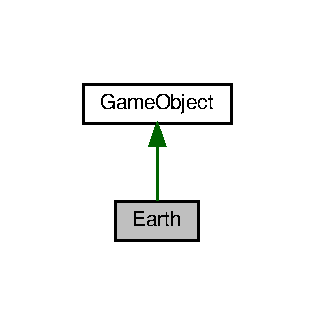
\includegraphics[width=151pt]{class_earth__coll__graph}
\end{center}
\end{figure}
\subsection*{Public Member Functions}
\begin{DoxyCompactItemize}
\item 
\mbox{\Hypertarget{class_earth_a9686e201e5d06af7befbe9c0d6b80e37}\label{class_earth_a9686e201e5d06af7befbe9c0d6b80e37}} 
{\bfseries Earth} (int x, int y, float scale)
\item 
\mbox{\Hypertarget{class_earth_add06e4af293b3723bf6ceae4c3c3834c}\label{class_earth_add06e4af293b3723bf6ceae4c3c3834c}} 
const sf\+::\+Sprite \& {\bfseries get\+Sprite} () const
\end{DoxyCompactItemize}
\subsection*{Additional Inherited Members}


The documentation for this class was generated from the following files\+:\begin{DoxyCompactItemize}
\item 
earth.\+h\item 
earth.\+cpp\end{DoxyCompactItemize}

\hypertarget{class_game_object}{}\section{Game\+Object Class Reference}
\label{class_game_object}\index{Game\+Object@{Game\+Object}}


Inheritance diagram for Game\+Object\+:
\nopagebreak
\begin{figure}[H]
\begin{center}
\leavevmode
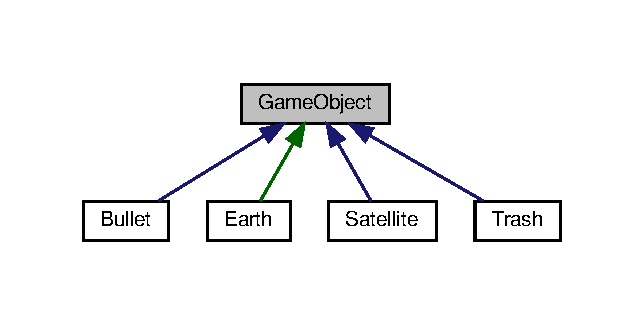
\includegraphics[width=309pt]{class_game_object__inherit__graph}
\end{center}
\end{figure}
\subsection*{Public Member Functions}
\begin{DoxyCompactItemize}
\item 
\mbox{\Hypertarget{class_game_object_a00106fe15899343de0805a7d7dc9d766}\label{class_game_object_a00106fe15899343de0805a7d7dc9d766}} 
{\bfseries Game\+Object} (int x, int y)
\item 
\mbox{\Hypertarget{class_game_object_aefb9850065652a0bb50c0e092aaacf59}\label{class_game_object_aefb9850065652a0bb50c0e092aaacf59}} 
int {\bfseries get\+X\+\_\+\+Null} ()
\item 
\mbox{\Hypertarget{class_game_object_a6c55dbb1345855d35bf8e4c00c8e8bd8}\label{class_game_object_a6c55dbb1345855d35bf8e4c00c8e8bd8}} 
int {\bfseries get\+Y\+\_\+\+Null} ()
\item 
\mbox{\Hypertarget{class_game_object_a13049dfd6703595d7e422cd7c9e80b47}\label{class_game_object_a13049dfd6703595d7e422cd7c9e80b47}} 
int {\bfseries is\+Alive} ()
\item 
\mbox{\Hypertarget{class_game_object_a0c2d5880f60a68cc6a191978094dfc66}\label{class_game_object_a0c2d5880f60a68cc6a191978094dfc66}} 
void {\bfseries kill\+Object} ()
\item 
\mbox{\Hypertarget{class_game_object_a8d45ee848362ff0c5b15f03e881486a6}\label{class_game_object_a8d45ee848362ff0c5b15f03e881486a6}} 
void {\bfseries alive\+Object} ()
\end{DoxyCompactItemize}
\subsection*{Protected Attributes}
\begin{DoxyCompactItemize}
\item 
\mbox{\Hypertarget{class_game_object_af6bddae0e71befe7cabe76c63c1cf5ea}\label{class_game_object_af6bddae0e71befe7cabe76c63c1cf5ea}} 
int {\bfseries x\+\_\+null}
\item 
\mbox{\Hypertarget{class_game_object_a681a040b87cf751ad9618f1013b0e7e6}\label{class_game_object_a681a040b87cf751ad9618f1013b0e7e6}} 
int {\bfseries y\+\_\+null}
\item 
\mbox{\Hypertarget{class_game_object_a94369b2b3bce43a9ff9655f5530c4f4a}\label{class_game_object_a94369b2b3bce43a9ff9655f5530c4f4a}} 
int {\bfseries is\+\_\+alive}
\end{DoxyCompactItemize}


The documentation for this class was generated from the following files\+:\begin{DoxyCompactItemize}
\item 
game\+\_\+obj.\+h\item 
game\+\_\+obj.\+cpp\end{DoxyCompactItemize}

\hypertarget{class_satellite}{}\section{Satellite Class Reference}
\label{class_satellite}\index{Satellite@{Satellite}}


Inheritance diagram for Satellite\+:
\nopagebreak
\begin{figure}[H]
\begin{center}
\leavevmode
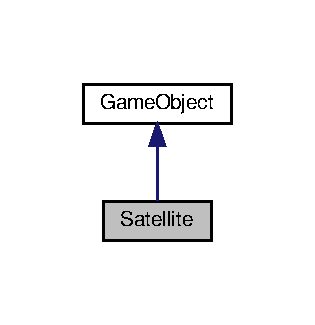
\includegraphics[width=151pt]{class_satellite__inherit__graph}
\end{center}
\end{figure}


Collaboration diagram for Satellite\+:
\nopagebreak
\begin{figure}[H]
\begin{center}
\leavevmode
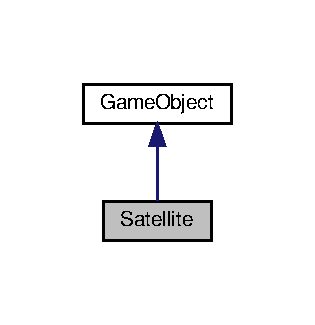
\includegraphics[width=151pt]{class_satellite__coll__graph}
\end{center}
\end{figure}
\subsection*{Public Member Functions}
\begin{DoxyCompactItemize}
\item 
\mbox{\Hypertarget{class_satellite_ae820a6cb0d5fb82912815ce2d12d6ead}\label{class_satellite_ae820a6cb0d5fb82912815ce2d12d6ead}} 
{\bfseries Satellite} (int x, int y, float scale)
\item 
\mbox{\Hypertarget{class_satellite_a8f3373cb1e63bc86ad9a93a838787b99}\label{class_satellite_a8f3373cb1e63bc86ad9a93a838787b99}} 
sf\+::\+Sprite \& {\bfseries get\+Sprite} ()
\item 
\mbox{\Hypertarget{class_satellite_a9672dcdd8e0a455e8a6225a161d2af2d}\label{class_satellite_a9672dcdd8e0a455e8a6225a161d2af2d}} 
float {\bfseries show\+Orbit} ()
\item 
\mbox{\Hypertarget{class_satellite_a8fd3c6d15b153bf2186fd9df46eb1572}\label{class_satellite_a8fd3c6d15b153bf2186fd9df46eb1572}} 
float \& {\bfseries get\+Orbit} ()
\item 
\mbox{\Hypertarget{class_satellite_adadcdf9164cf336687b1af7afce19a92}\label{class_satellite_adadcdf9164cf336687b1af7afce19a92}} 
float {\bfseries show\+Delta} () const
\item 
\mbox{\Hypertarget{class_satellite_a173a28416bfdb020084ff4502d5bb983}\label{class_satellite_a173a28416bfdb020084ff4502d5bb983}} 
float \& {\bfseries get\+Delta} ()
\item 
\mbox{\Hypertarget{class_satellite_ad19d99087f6683d1bf5df900dafa3e38}\label{class_satellite_ad19d99087f6683d1bf5df900dafa3e38}} 
float {\bfseries show\+Beta} ()
\item 
\mbox{\Hypertarget{class_satellite_add23f290f62fa2af6d650b13d6919708}\label{class_satellite_add23f290f62fa2af6d650b13d6919708}} 
float \& {\bfseries get\+Beta} ()
\end{DoxyCompactItemize}
\subsection*{Additional Inherited Members}


The documentation for this class was generated from the following files\+:\begin{DoxyCompactItemize}
\item 
satellite.\+h\item 
satellite\+\_\+obj.\+cpp\end{DoxyCompactItemize}

\hypertarget{class_trash}{}\section{Trash Class Reference}
\label{class_trash}\index{Trash@{Trash}}


Inheritance diagram for Trash\+:
\nopagebreak
\begin{figure}[H]
\begin{center}
\leavevmode
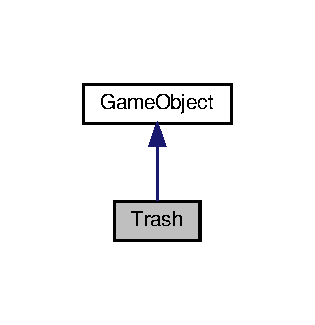
\includegraphics[width=151pt]{class_trash__inherit__graph}
\end{center}
\end{figure}


Collaboration diagram for Trash\+:
\nopagebreak
\begin{figure}[H]
\begin{center}
\leavevmode
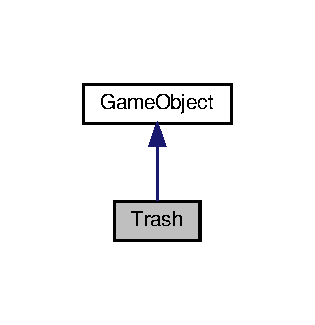
\includegraphics[width=151pt]{class_trash__coll__graph}
\end{center}
\end{figure}
\subsection*{Public Member Functions}
\begin{DoxyCompactItemize}
\item 
\mbox{\Hypertarget{class_trash_a8c43bbea8527c8f661b92fc4c51dff10}\label{class_trash_a8c43bbea8527c8f661b92fc4c51dff10}} 
{\bfseries Trash} (int x, int y, float scale)
\item 
\mbox{\Hypertarget{class_trash_a3a7569c9c8542a92a484d767244d0718}\label{class_trash_a3a7569c9c8542a92a484d767244d0718}} 
sf\+::\+Circle\+Shape \& {\bfseries get\+Circle} ()
\item 
\mbox{\Hypertarget{class_trash_acc41ec490091c10b2052a1666f581d84}\label{class_trash_acc41ec490091c10b2052a1666f581d84}} 
sf\+::\+Sprite \& {\bfseries get\+Sprite} ()
\item 
\mbox{\Hypertarget{class_trash_a26ad6b9e1ee2efe962371263fe2ce8e5}\label{class_trash_a26ad6b9e1ee2efe962371263fe2ce8e5}} 
int {\bfseries get\+CircleX} ()
\item 
\mbox{\Hypertarget{class_trash_a7c412d5f2a659cefb019a1f13f32bab8}\label{class_trash_a7c412d5f2a659cefb019a1f13f32bab8}} 
int {\bfseries get\+CircleY} ()
\end{DoxyCompactItemize}
\subsection*{Additional Inherited Members}


The documentation for this class was generated from the following files\+:\begin{DoxyCompactItemize}
\item 
trash.\+h\item 
trash\+\_\+obj.\+cpp\end{DoxyCompactItemize}

%--- End generated contents ---

% Index
\backmatter
\newpage
\phantomsection
\clearemptydoublepage
\addcontentsline{toc}{chapter}{Index}
\printindex

\end{document}
